
	\documentclass{article}
	\usepackage{amsmath,amssymb}
	\usepackage[inline]{enumitem}
	\usepackage{blindtext}
	\usepackage{booktabs}
	\usepackage{graphicx}
	\usepackage{xcolor}
	\usepackage[vmargin = 1.5in, top = 1in, bottom = 1.2in, letterpaper]{geometry}
	\usepackage{listings}
	\usepackage{courier}
	\usepackage{bm}
	\lstset{
	basicstyle = \small\tt,
	keywordstyle = \tt\color{blue},
	commentstyle = \it\color[cmyk]{1,0,1,0},
	stringstyle = \tt\color[RGB]{128,0,0},
	%frame = single,
	backgroundcolor = \color[RGB]{245,245,244},
	breaklines,
	extendedchars = false,
	xleftmargin = 2em,
	xrightmargin = 2em,
	aboveskip = 1em,
	tabsize = 4,
	showspaces = false
	}
	\begin{document}
	
	% \newfontfamily\courier{Courier New}

	
	\title{STAT 500 Homework 9}
	\author{Yifan Zhu}
	\maketitle
	
	\begin{enumerate}[leftmargin = 0 em, label = \arabic*., font = \bfseries]
	\item

		The simple linear regression model for this problem is:
		\[Y_i = \beta_0 + \beta_1 x_i + \epsilon\]
		The parameter $\beta_0$ is the mean price of diamonds that have
a weight of 0 g.

The parameter $\beta_1$ is the change in the mean price of diamonds for a 1 g increase in weight.

The parameter $\sigma^2$ is the variance in price of diamonds that
all have the same weight.

\item \

\begin{center}
	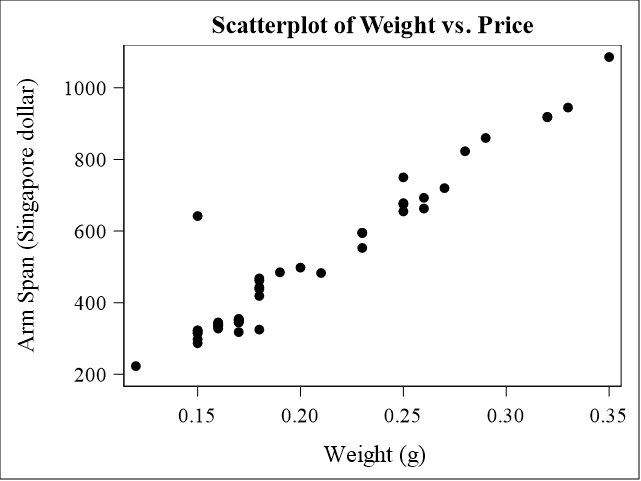
\includegraphics[width = 0.6\textwidth]{scatter.png}
\end{center}
The relationship between the two variables is positive and appears to be linear. The points
in the scatterplot are generally close to a line.


\item 
\[\hat{Y_i}  = -229.94174 + 3612.49521 x_i\]


\item Here is the ANOVA Table from the SAS output.

\begin{center}
	\begin{tabular}{llllll}
\toprule
Source&DF&Sum of Squares&Mean Square&F Value&Pr $>$ F\\
\midrule
Model&1&1986120&1986120&574.20&$<.0001$\\
Error&46&159112&3458.95446&&\\
Corrected Total&47&2145232&&&\\
\bottomrule
\end{tabular}
\end{center}
The test of significance of the slope of the linear regression model is:
\[H_0 : \beta_1 = 0,\, H_a : \beta_1 \neq 0\]
The test statistic from the ANOVA Table is F = 574.20 with a p-value $<$ 0.0001. So we
will reject the null hypothesis and conclude the slope in the linear regression model is
non-zero. Weight is statistically significant predictor of price in this population of
diamonds.

\item 
From the ANOVA Table, we have 
\[R^2 = \frac{SS_{model}}{SS_{total}} = 0.9258\]
This means that 92.58\% of the variation in the price of these diamonds can be
explained by the linear regression model with weight.


\item 
From the SAS output, this confidence interval is located in the table under the column 95\%
CL Mean. For a height of 0.2 g, the value of this confidence interval is \textbf{(475.4583, 509.6563)}. 
This means we are 95\% confident the mean price of all diamonds that are 0.2 g is between 475.4583 and 509.6563 Singapore dollars.


\item 
From the SAS output, this confidence interval is is located in the table under the column 95\% CL Predict. For a weight of 0.3 g, the value
of this confidence interval is \textbf{(730.5604, 977.0533)}. This means we would predict, with 95\% confidence, the price of a diamonds that are 0.3 g would
be between 730.5604 and 977.0533 Singapore dollars. 


\item 
\begin{itemize}
	\item 
	Independence cannot generally be checked through any graphs or statistics. Random sample from a population is not mentioned in the description, we cannot
conclude the observations are independent or not.

\item
Normality of the error terms can be checked through the normal quantile plot. In the normal quantile plot, the residuals appear to follow a
straight line except for one outlier.  This would indicate the data follow the assumption fairly well.

\begin{center}
	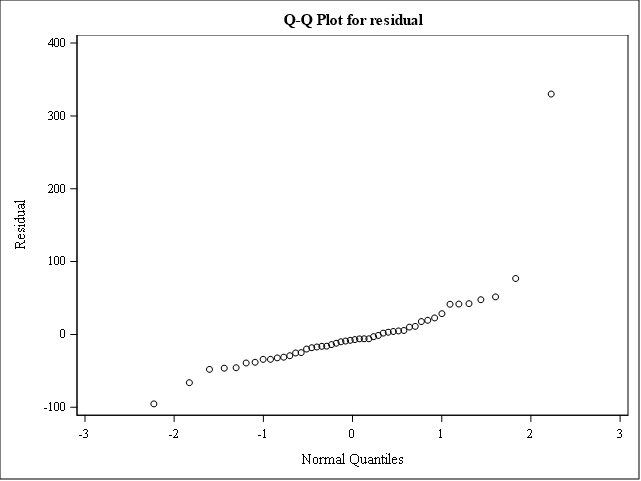
\includegraphics[width = 0.6\textwidth]{qq.png}
\end{center}

\item
Homogeneous variance can be checked through the residual plot. From the plot we can see except for one outlier the residual does not depend on the value of the explanatory variable
weight. 

\item
Linearity can also be checked through the residual plot. There
does not appear to be a pattern in the residual plot that would indicate another type of
relationship between price and weight other than linear.

\begin{center}
	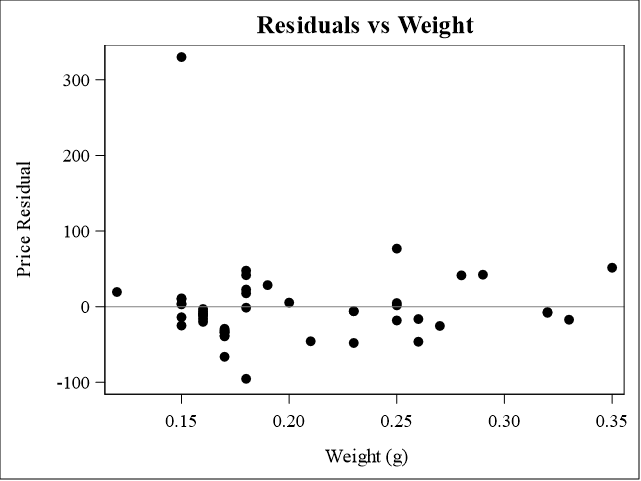
\includegraphics[width = 0.6\textwidth]{res.png}
\end{center}

\item
Since there is only one outlier, it will not affect the result too much.
\end{itemize}



\end{enumerate}

	\end{document}